\documentclass[10pt]{article}
\usepackage{icmlko}

\icmlmeta{IP 파운데이션 월드모델}{347}{서랍 속의 축}{노트 309 에서 검사 셋을 다 통과한 축이 열여덟 노트 동안 서랍에 있었다 --- 꺼내니 펀딩이 $+$0.096 다}

\begin{document}

\twocolumn[
\icmlheader

\begin{abstract}
노트 346이 ``다른 쟀는데 안 쓴 것 --- 이번이 처음이 아닐 것''을 갈래로
남겼다. 훑었다. \textbf{있다.}

\texttt{fund\_cat} 은 노트 309에서 \textbf{채택 검사 셋을 다 통과한 첫
축}이었다(크루스칼 H$=$56.7 · 시간 조각 5/5 · 잔차 H$=$42.2). 그때 판이
$+$0.0023 이었고 노트 329가 올바른 가중으로 다시 재니 짝지은 차
$+$0.0017(12/14)로 부호가 섰다. \textbf{그런데 축 세트
\texttt{trendcalwikitagfund} 로만 있고 챔피언에는 한 번도 안 들어갔다.}

\textbf{지금 판에서 다시 쟀다.}

\begin{center}\small
\begin{tabular}{lrr}
\hline
 & 검사 ⑤ & 실제 \\
\hline
판 & $+$0.0035 (8/8) & \textbf{$+$0.0030} (11/12) \\
펀딩 & $+$0.0981 (8/8) & \textbf{$+$0.0964} (12/12) \\
\hline
\end{tabular}
\end{center}

\textbf{펀딩이 0.2514 에서 0.3846 이다} --- 이 창에서 아이돌 다음으로 큰
도메인 이득이고, 새 자료도 새 축도 아니다. \textbf{열여덟 노트 전에 만들어
둔 것을 꺼낸 것뿐이다.}

배포 규칙 ①②를 통과한다(제일 나쁜 아이돌 $-$0.0172 · $t{\approx}0.31$).
\textbf{챔피언에 넣었다 --- 판 0.4729 $\to$ 0.4763.}

\textbf{그리고 검사 ⑤ 가 세 번째로 맞혔다.}

\begin{center}\footnotesize
\begin{tabular}{lrr}
\hline
 & 검사 ⑤ & 실제 \\
\hline
모바일 태그(343) & $+$0.0042 & $+$0.0041 \\
세계애니 장르(344) & $+$0.0027 & $+$0.0015 \\
\textbf{fund\_cat}(347) & $+$0.0035 & $+$0.0030 \\
\hline
\end{tabular}
\end{center}
\end{abstract}
]

\section{서랍을 열었다}

\begin{center}\footnotesize
\begin{tabular}{lll}
\hline
축 세트 & 무엇 & 판(그때) \\
\hline
\texttt{...fund} & \texttt{fund\_cat}(309) & $+$0.0023 \\
\texttt{...ani} & \texttt{anime\_medium}(321) & $+$0.0000 \\
\texttt{...raw} & 원천 축 열(324) & $-$0.0027 \\
\hline
\end{tabular}
\end{center}

셋 중 \texttt{fund\_cat} 만 양수였고 셋 다 챔피언 밖에 있었다.
\textbf{양수인 것을 안 넣은 채로 열여덟 노트가 지났다.}

\begin{figure*}[t]
\centering
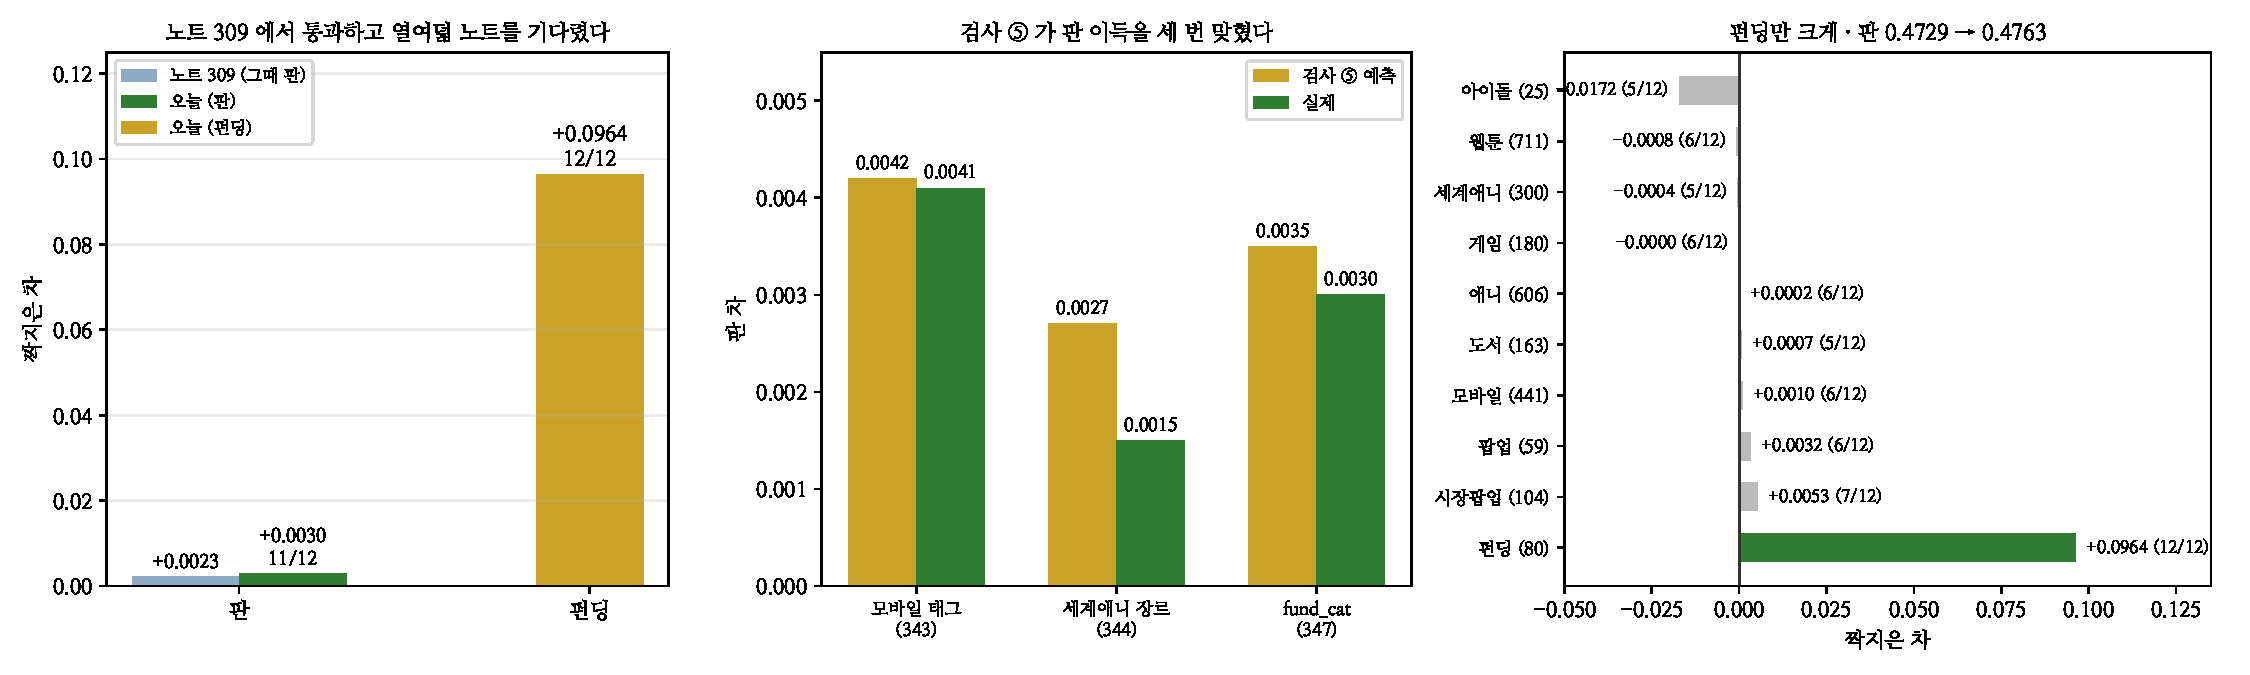
\includegraphics[width=\textwidth]{figs/fund.pdf}
\caption{왼쪽 --- 노트 309와 오늘. 가운데 --- 검사 ⑤ 세 번.
오른쪽 --- 도메인별.}
\end{figure*}

\section{지금 재면 훨씬 크다}

\begin{center}\footnotesize
\begin{tabular}{lrrr}
\hline
 & 평균 & SD & 양수 \\
\hline
\textbf{펀딩} & \textbf{$+$0.0964} & 0.0223 & \textbf{12/12} \\
시장팝업 & $+$0.0053 & 0.0297 & 7/12 \\
팝업 & $+$0.0032 & 0.0092 & 6/12 \\
아이돌 & $-$0.0172 & 0.0297 & 5/12 \\
\hline
\textbf{판} & \textbf{$+$0.0030} & 0.0017 & \textbf{11/12} \\
\hline
\end{tabular}
\end{center}

\textbf{펀딩 기준값이 0.2514 $\to$ 0.3846 이다.} 노트 309가 잰 판
$+$0.0023 은 도메인 이득을 안 적었는데, \textbf{펀딩이 판의 3.0\%라
$+$0.096 이 판에 $+$0.003 으로 들어온다.} 그때도 지금도 판으로는 작고
도메인으로는 크다.

\paragraph{왜 그때 안 넣었나} 노트 309는 축을 \emph{만든} 노트였고
판정치는 판 $\rho$ 다. $+$0.0023 은 그때 미결정 폭 0.010 안이라
``못 가른다''로 읽혔고, \textbf{못 가르는 것은 안 넣는다}가 안전한
기본값처럼 보였다. \textbf{그런데 도메인 이득을 같이 보지 않았다.}

\section{검사 ⑤ 가 세 번 맞혔다}

\begin{center}\footnotesize
\begin{tabular}{lrrr}
\hline
후보 & 검사 ⑤ & 실제 & 차 \\
\hline
모바일 태그 & $+$0.0042 & $+$0.0041 & 0.0001 \\
세계애니 장르 & $+$0.0027 & $+$0.0015 & 0.0012 \\
fund\_cat & $+$0.0035 & $+$0.0030 & 0.0005 \\
\hline
\end{tabular}
\end{center}

\textbf{셋 다 방향이 맞고 둘은 소수 넷째 자리에서 만난다.} 노트 344가
``두 사례로는 못 말한다''고 했는데 셋째가 붙었다 --- \textbf{검사 ⑤ 는
붙이기 전에 판 이득을 어림하는 데 쓸 수 있다.} 뽑기 여덟(적합 열여섯)이
드는 값이다.

\section{남은 것}
\begin{center}\footnotesize
\begin{tabular}{ll}
\hline
갈래 & 왜 \\
\hline
\textbf{서랍을 마저} & \texttt{ani} · \texttt{raw} 도 지금 재면 \\
판정치에 도메인을 & 판만 보면 서랍이 또 생긴다 \\
아이돌이 왜 또 $-$0.017 & 남의 축인데 내려간다 \\
검사 ⑤ 를 자동으로 & 세 번 맞혔으면 규약에 \\
\hline
\end{tabular}
\end{center}

\paragraph{규약} \textbf{``못 가른다''는 ``안 넣는다''가 아니다.} 노트 309가
\texttt{fund\_cat} 을 판 $+$0.0023 으로 재고 미결정 폭 안이라 그냥 뒀다.
\textbf{그런데 미결정 폭은 판정치에 대한 것이지 채택에 대한 것이 아니다}
--- 배포 규칙은 ``폭 안이면 배포가 정한다''이고, 여기서 배포가 정할 근거는
\emph{도메인 이득}이었는데 그것을 안 봤다. \textbf{판이 못 가르면 도메인을
보라} --- 안 그러면 잰 것이 서랍에 쌓인다.

\end{document}
